%%!TEX TS-program = pdflatexmk
%%!TEX encoding = UTF-8 Unicode
\documentclass[11pt]{article}
\usepackage[utf8]{inputenc}
\usepackage[T1]{fontenc}
\usepackage[french]{babel}

\usepackage[letterpaper,body={6.0in,9.5in},vmarginratio=1:1]{geometry}
\usepackage[small,compact]{titlesec}

\usepackage{fourier}
\usepackage[scaled=0.85]{berasans}
\usepackage[scaled=0.85]{beramono}
\usepackage{microtype}

\usepackage{graphicx}
\usepackage{xcolor}
\usepackage[colorlinks, urlcolor=darkgray, linkcolor=darkgray]{hyperref}

\usepackage{booktabs}


%\usepackage{applekeys}
% Alternate Special Keys 
\newcommand{\optkey}{\texttt{Opt}}
\newcommand{\ctlkey}{\texttt{Ctl}}
\newcommand{\cmdkey}{\texttt{Cmd}}
\newcommand{\esckey}{\texttt{Esc}}
\newcommand{\tabkey}{\texttt{Tab}}
\newcommand{\shiftkey}{\texttt{Shift}}

\newcommand{\mnu}[1]{\texttt{#1}}
\newcommand{\cmd}[1]{\texttt{#1}}
\newcommand{\To}{\,\(\to\)\,}

%\pagestyle{empty}

% set | as a command character within verbatim so you can execute commands there
\usepackage{verbatim}
\makeatletter
\addto@hook\every@verbatim{\catcode`|=0}
\makeatother

% define colored items to be inserted in verbatim environments
\setlength{\fboxsep}{0pt}
\newcommand{\selmark}{\colorbox{cyan}{\rule[-0.5ex]{0ex}{2.1ex}\texttt{•}}}
\newcommand{\selcom}{\colorbox{cyan}{\rule[-0.5ex]{0ex}{2.1ex}\texttt{•‹comment›}}}
\newcommand{\selcombwra}{\colorbox{cyan}{\rule[-0.5ex]{0ex}{2.1ex}\texttt{•‹placement: r,R,l,L,i,I,o,O›}}}
\newcommand{\selcomrulewidth}{\colorbox{cyan}{\rule[-0.5ex]{0ex}{2.1ex}\texttt{•‹width›}}}
\newcommand{\selcomrulelift}{\colorbox{cyan}{\rule[-0.5ex]{0ex}{2.1ex}\texttt{•‹lift›}}}

% define a few items for easy use
\newcommand{\fastex}{Fas\hspace{-.15em}\TeX}
\newcommand{\TS}{\textsf{\TeX Shop}}
\newcommand{\TSVersion}{2.30}
\newcommand{\CCT}{\texttt{CommandCompletion.txt}}

\title{Complètement de commande\\ avec \TS\ 6+\\ pour l’impatient}
\author{Herbert Schulz\thanks{Traduit par René Fritz le 26 décembre 2016 ; mis à jour pour \TS\ 6 en novembre 2026.}\\\small\href{mailto:herbs2@mac.com}{herbs2@mac.com}}
\date{2026/11/18}

\begin{document}
\maketitle
\thispagestyle{empty}

\section*{Introduction}

Le balisage de \LaTeX\ est plutôt prolixe, ce qui est agréable, car il décrit ce qu’il est censé faire, mais un peu pénible à écrire. Le complètement de commande vous permet d’insérer des environnements complets et des commandes en quelques frappes suivies d’une pression sur la touche de «~déclenchement~» (qui est, par défaut, \cmd{Esc} mais peut être remplacée par \cmd{Tab} dans \mnu{TeXShop}\To\mnu{Réglages}\To\mnu{Clavier}).

Les commandes avec arguments ont généralement un repère (\texttt{•}) placé à la place de chaque argument. Pour aller à l’argument suivant, utilisez la commande \mnu{Édition}\To\mnu{Repères}\To\mnu{Repère suivant} (\cmd{Ctl-Cmd-F} [ou \cmd{Opt-déclenchement}]). Ceci sélectionne en même temps le repère, pour qu’il soit automatiquement remplacé par l’information saisie. Voir la documentation complète, avec les listes de commandes et d’abréviations fournies avec \TS, dans le dossier \path{~/Library/TeXShop/CommandCompletion/}, pour plus d’informations. Vous pouvez ouvrir \path{~/Library/TeXShop} avec la commande \mnu{Ouvrir \textasciitilde/Bibliothèque/TeXShop} du menu \mnu{TeXShop}.

\section*{Utilisation}

Un grand nombre de commandes et d’environnements peuvent être facilement complétés en entrant soit le début de la commande, soit l’une des abréviations de ces commandes ou environnements. Les exemples qui suivent sont là pour vous aider à démarrer.

Bien que la liste des abréviations soit assez vaste, il vous suffira d’apprendre celles que vous utilisez souvent et de retenir progressivement les autres au fur et à mesure de vos besoins. En outre, il suffit d’appuyer plusieurs fois sur la touche de déclenchement pour obtenir les mêmes commandes ou environnements avec un nombre différent d’options, etc.

\subsection*{Complètement de commande}

Vous pouvez compléter de nombreuses commandes en commençant à les saisir puis en appuyant sur la touche de déclenchement. Les variantes qui diffèrent par leur nombre d’arguments optionnels sont générées par des pressions successives sur la touche de déclenchement. Ainsi, taper \verb|\sec| sur une nouvelle ligne, puis la touche de déclenchement, produit
\begin{verbatim}
\section{|selmark}
\end{verbatim}
tandis qu’une seconde pression sur la touche de déclenchement donne
\begin{verbatim}
\section*{|selmark}
\end{verbatim}
la variante étoilée, et qu’une dernière pression de cette touche donne
\begin{verbatim}
\section[|selmark]{•}
\end{verbatim}
avec l’argument optionnel.

\subsection*{Abréviations}

Outre le complètement des commandes entrées partiellement, il y a aussi de nombreuses abréviations. Celles-ci sont de courts mnémoniques pour accéder à des substitutions complètes.

Toutes les abréviations d’environnements commencent par un «~\texttt{b}~». Pour obtenir l’environnement \cmd{itemize} complet, entrez \verb|\bite| seul sur une ligne et appuyez sur la touche de déclenchement, ce qui produira
\begin{verbatim}
\begin{itemize}
\item
|selmark
\end{itemize}•
\end{verbatim}
terminé par un repère supplémentaire pour que vous puissiez facilement accéder à la fin de l’environnement. Des items supplémentaires peuvent être créés en tapant \verb|\it| puis la touche de déclenchement afin d’obtenir
\begin{verbatim}
\item
|selmark
\end{verbatim}
prêt pour l’entrée d’un texte.

En plus de la commande \verb|\section|, les commandes de sectionnement de niveau inférieur possèdent leurs abréviations. Les sous-sections peuvent être obtenues en tapant \verb|\ssec| puis en appuyant sur la touche de déclenchement, ce qui donnera
\begin{verbatim}
\subsection{|selmark}
\end{verbatim}
et des pressions successives sur la touche de déclenchement donneront la variante étoilée puis, enfin, la variante avec l’argument optionnel.

En dernier exemple, \verb|\tt| suivi de la touche de déclenchement donne la commande \verb|\texttt{|\selmark\verb|}|, et une seconde pression de cette touche donne la déclaration \verb|\ttfamily| ; des résultats similaires sont obtenus avec les autres commandes de changement de police.

\subsection*{Aide-mémoire}

Il est facile de se souvenir des arguments des commandes utilisées assez souvent, mais pas de celles qui le sont rarement ; ces dernières sont tout indiquées pour les aide-mémoire. L’ordre des arguments de la commande \verb|\rule| en est un exemple : tapez \verb|\rul| et la touche de déclenchement pour obtenir
\begin{verbatim}
\rule{|selcomrulewidth}{•‹height›}
\end{verbatim}
et une pression supplémentaire de la touche de déclenchement donne
\begin{verbatim}
\rule[|selcomrulelift]{•‹width›}{•‹height›}
\end{verbatim}
la version avec l’argument optionnel. Un autre exemple est l’environnement \texttt{wrapfigure} de l’extension \texttt{wrapfig}, qui dispose de plusieurs versions différant par le nombre et la position des arguments optionnels. Pour voir les variantes avec les aide-mémoire, tapez \verb|\bwr| sur une ligne vide et appuyez sur la touche de déclenchement pour obtenir
\begin{verbatim}
\begin{wrapfigure}{|selcombwra}{•‹width›}
•
\end{wrapfigure}•
\end{verbatim}
les versions avec arguments optionnels venant aux pressions suivantes de la touche de déclenchement.

\section*{Taper \cmd{\textbackslash} est parfois compliqué}

Avec certains claviers, il est fastidieux d’entrer directement le caractère «~\verb|\|~» : par exemple, sur un clavier français, il faut actionner plusieurs touches. Mais tout espoir n’est pas perdu ! Dans la plupart des cas, il n’est pas nécessaire de commencer une abréviation ou un début de commande par un «~\verb|\|~», mais plutôt par n’importe quel «~caractère blanc~» (c’est-à-dire le début d’une nouvelle ligne, une espace ou une tabulation). Donc, au lieu de
\begin{verbatim}
\sec
\end{verbatim}
puis la touche de déclenchement pour produire
\begin{verbatim}
\section{|selmark}
\end{verbatim}
vous pouvez utiliser
\begin{verbatim}
sec
\end{verbatim}
au début d’une ligne et la touche de déclenchement produira la même commande.

De même, entrer \verb|tt| suivi de la touche de déclenchement donne \verb|\texttt{|\selmark\verb|}|, car il est précédé d’une espace. Mais \verb|`tt| ne fonctionnera \emph{pas}, puisque \verb|tt| \emph{n’est pas} précédé d’un «~caractère blanc~» ; dans ce cas, vous devrez utiliser \verb|`\tt|. Le plus simple, pour se faciliter la tâche, est de créer une macro qui ne fait qu’insérer un «~\verb|\|~» (sans les guillemets) et de l’associer à un raccourci simple avec la touche \mnu{Cmd}.

\section*{Hé, les exemples ne marchent pas !}

Si ces exemples ne fonctionnent pas, c’est probablement que vous devez laisser \TS\ mettre à jour le dossier \path{~/Library/TeXShop/CommandCompletion/} ; supprimez simplement ce dossier de \path{~/Library/TeXShop/} et redémarrez \TS.

\section*{Tables des commandes et environnements fournis}

Cette section contient une liste, que l’on espère complète, des commandes et abréviations fournies dans \CCT. Elle est divisée en environnements, commandes et déclarations, et lettres grecques. Si vous saisissez le début d’une abréviation, la recherche commence à la première correspondance, et des pressions successives sur \esckey\ parcourent la liste tant qu’il y a une correspondance ; par exemple, si vous tapez \texttt{be}, des pressions successives sur \esckey\ donneront \texttt{benu}, \texttt{benuo}, \texttt{bequ}, \texttt{bequs}, \texttt{beqn} et \texttt{beqns} avant de revenir au \texttt{be} initial. En ajoutant des lettres à l’abréviation, vous atteindrez le complètement voulu avec moins de pressions sur \esckey. En réalité, certaines commandes et déclarations sont dispersées parmi les environnements dans le fichier \CCT, si bien qu’il peut parfois y avoir des éléments supplémentaires. Les tables n’indiquent ni les complètements ordinaires ni les versions des abréviations commençant par «~\verb"\"~».

\textbf{À nouveau : la liste peut paraître un peu intimidante. Inutile de «~mémoriser~» toutes ces abréviations ; apprenez-en le minimum, au fur et à mesure de vos besoins. De plus, les variantes d’une abréviation s’obtiennent par des pressions successives sur \esckey ; voir par exemple la figure~\ref{fig:sec}.}
\begin{figure}\centering
\makebox[\textwidth]{
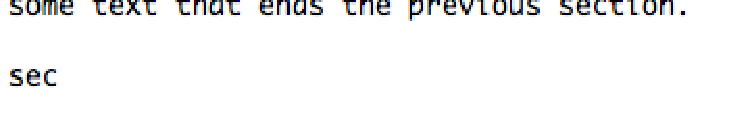
\includegraphics[width=3in]{figs/startsec}
\hfill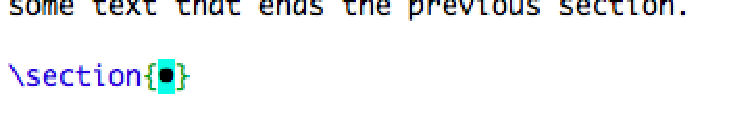
\includegraphics[width=3in]{figs/sec}}
\makebox[\textwidth]{
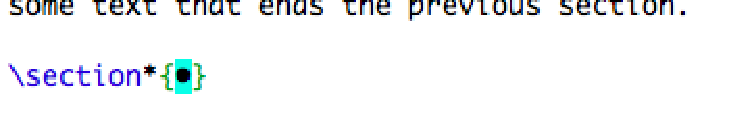
\includegraphics[width=3in]{figs/secs}
\hfill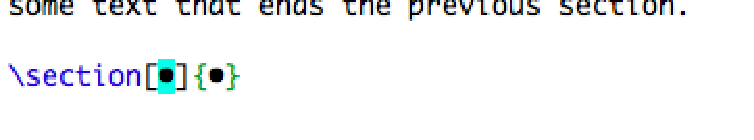
\includegraphics[width=3in]{figs/seco}}
\caption{Saisie initiale de \texttt{sec} puis pressions successives sur \esckey, du début jusqu’au dernier résultat avant le retour au début. Correspond à la suite \texttt{début}\(\to\)\texttt{sec}\(\to\)\texttt{secs}\(\to\)\texttt{seco}.}
\label{fig:sec}
\end{figure}

\subsection*{Abréviations d’environnements}

La table~\ref{tbl:environments}, page~\pageref{tbl:environments}, contient la liste des abréviations des différents environnements fournies dans \CCT. Plusieurs environnements voisins verticalement et de (presque) même nom correspondent à des variantes qui diffèrent par le nombre et la répartition des arguments optionnels, ou à des variantes étoilées. Un même environnement peut aussi avoir plusieurs abréviations.

\subsection*{Commandes et déclarations}

Comme pour les environnements, il existe de nombreuses variantes avec options et variantes étoilées, ainsi que plusieurs abréviations pour une même commande. Voir la table~\ref{tbl:commands}, page~\pageref{tbl:commands}.

\subsection*{Lettres grecques}

Les abréviations des lettres grecques figurent dans la table~\ref{tbl:greek}, page~\pageref{tbl:greek}. Il existe des versions en «~\texttt{dx}~» (au lieu de «~\texttt{x}~» seul) des lettres grecques, destinées à être insérées dans le texte : \texttt{dxa} suivi de \esckey\ produit \verb'\(\alpha\)' dans la source et \(\alpha\) dans une ligne de texte composée. Ces versions en «~\texttt{d}~», pour les formules dans le texte, ne figurent pas dans la table.

\begin{table}[!h]
\small
\centering
\caption{Abréviations d’environnements fournies dans \CCT.}
\label{tbl:environments}
\vspace{10pt}
\begin{tabular}{llll}
\textbf{Abréviation} & \textbf{Environnement} & \textbf{Abréviation} & \textbf{Environnement} \\
\cmidrule[0.5pt](lr){1-1} \cmidrule[0.5pt](lr){2-2} \cmidrule[0.5pt](lr){3-3} \cmidrule[0.5pt](lr){4-4}\\
barr      & array       & blett   & letter \\
babs      & abstract    & blist   & list \\
bali      & align       & bminp   & minipage \\
balis     & align*      & bminpo  & minipage \\
baliat    & alignat     & bmult   & multline \\
baliats   & alignat*    & bmults  & multline* \\
balied    & aligned     & bpict   & picture \\
baliedat  & alignedat   & bpmat   & pmatrix \\
baliedato & alignedat   & bquot   & quotation \\
bapp      & appendix    & bquo    & quote \\
bbmat     & bmatrix     & bsplit  & split \\
bcase     & cases       & bsubeq  & subequations \\
bcent     & center      & btab    & tabular \\
bcenum    & compactenum & btabs   & tabular* \\
bcenumo   & compactenum & btabx   & tabularx \\
bcitem    & compactitem & btabl   & table \\
bcitemo   & compactitem & btablo  & table \\
bdes      & description & btabls  & table* \\
benu      & enumerate   & btablso & table* \\
benuo     & enumerate   & btbl    & table \\
bequ      & equation    & btblo   & table \\
bequs     & equation*   & btbls   & table* \\
beqn      & eqnarray    & btblso  & table* \\
beqns     & eqnarray*   & btabb   & tabbing \\
bfig      & figure      & bbib    & thebibliography \\
bfigo     & figure      & bindex  & theindex \\
bframe    & frame       & btheo   & theorem \\
bframeo   & frame       & btitpg  & titlepage \\
bflalig   & flalign     & btrivl  & trivlist \\
bflaligs  & flalign*    & bvarw   & varwidth \\
bfll      & flushleft   & bverb   & verbatim \\
bflr      & flushright  & bvers   & verse \\
bgath     & gather      & bwrap   & wrapfigure \\
bgaths    & gather*     & bwrapo  & wrapfigure \\
bgathed   & gathered    & bwrapo2 & wrapfigure \\
bgathedo  & gathered    & bwrapoo & wrapfigure \\
bite      & itemize     &         & \\
biteo     & itemize     &         & \\
\end{tabular}
\end{table}

\begin{table}[!h]
\small
\centering
\caption{Commandes et déclarations dans \CCT.}
\label{tbl:commands}
\vspace{10pt}
\makebox[\textwidth]{%
\begin{tabular}{llllll}
\textbf{Abréviation} & \textbf{Commande} & \textbf{Abréviation} & \textbf{Commande} & \textbf{Abréviation} & \textbf{Commande} \\
\cmidrule[0.5pt](lr){1-1} \cmidrule[0.5pt](lr){2-2} \cmidrule[0.5pt](lr){3-3} \cmidrule[0.5pt](lr){4-4} \cmidrule[0.5pt](lr){5-5} \cmidrule[0.5pt](lr){6-6}
\texttt{-{}-}    & textendash        & midr       & midrule        & renewcomo       & renewcommand \\
\texttt{-{}-{}-} & textemdash        & mnorm      & mathnormal     & renewcomoo      & renewcommand \\
\texttt{-{}-{}-} & textemdash avec esp.   & msf        & mathsf         & rncm            & renewcommand \\
adlen            & addtolength       & mtt        & mathtt         & rnewc           & renewcommand \\
adcount          & addtocounter      & mit        & mathit         & rncmo           & renewcommand \\
bf               & textbf            & midr       & midrule        & rnewcoo         & renewcommand \\
bfd              & bfseries          & mnorm      & mathnormal     & rncmoo          & renewcommand \\
biblio           & bibliography      & mdd        & mdseries       & rmc             & rmfamily \\
bibstyle         & bibliographystyle & mbox       & mbox           & rbox            & raisebox \\
botr             & bottomrule        & makebox    & makebox        & rboxo           & raisebox \\
bibitem          & bibitem           & mboxo      & makebox        & rboxoo          & raisebox \\
bibitemo         & bibitem           & makebox    & makebox        & sec             & section \\
center           & centering         & mboxoo     & makebox        & secs            & section* \\
chap             & chapter           & mpar       & marginpar      & seco            & section \\
cmidr            & cmidrule          & multic     & multicolumn    & ssec            & subsection \\
cmidro           & cmidrule          & ncol       & espace \& espace & ssecs           & subsection* \\
em               & emph              & ncm        & newcommand     & sseco           & subsection \\ 
emd              & em                & newc       & newcommand     & sssec           & subsubsection \\
foot             & footnote          & ncmo       & newcommand     & sssecs          & subsubsection* \\
frac             & frac              & newco      & newcommand     & ssseco          & subsubsection \\
fbox             & fbox              & ncmoo      & newcommand     & spar            & subparagraph \\
fboxo            & framebox          & newcoo     & newcommand     & spars           & subparagraph* \\
fboxoo           & framebox          & nct        & newcolumntype  & sparo           & subparagraph \\
geometry         & geometry          & newct      & newcolumntype  & setl            & setlength \\
hw               & headwidth         & newpg      & newpage        & stcount         & stepcounter \\
hw2tw            & headw\(=\)textw   & npg        & newpage        & sf              & textsf \\
href             & href              & nline      & newline        & sfd             & sffamily \\
item             & item              & newlin     & newline        & sc              & textsc \\
ito              & item              & nlen       & newlength      & scd             & scshape \\
incg             & includegraphics   & newlen     & newlength      & sl              & textsl \\
incgo            & includegraphics   & nenv       & newenvironment & sld             & slshape \\
it               & textit            & newenv     & newenvironment & sqrt            & sqrt \\
itd              & itshape           & nenvo      & newenvironment & sqrto           & sqrt \\
latex            & LaTeX             & newenvo    & newenvironment & tt              & texttt \\
latexs           & LaTeX avec esp.        & nenvoo     & newenvironment & ttd             & ttfamily \\
latexe           & LaTeXe            & newenvoo   & newenvironment & tw              & textwidth \\
latexes          & LaTeXe avec esp.       & pgref      & pageref        & tex             & TeX \\
label            & label             & par        & paragraph      & texs            & TeX avec esp. \\
lbl              & label             & pars       & paragraph*     & tilde           & textasciitilde \\
lettrine         & lettrine          & paro       & paragraph      & topr            & toprule \\
lettrineo        & lettrine          & pgs        & pagestyle      & toc             & tableofcontents \\
listf            & listoffigures     & parbox     & parbox         & tableofcontents & tableofcontents \\
listt            & listoftables      & parboxo    & parbox         & tpgs            & thispagestyle \\
rule             & rule              & parboxoo   & parbox         & thispagestyle   & thispagestyle \\
ruleo            & rule              & parboxooo  & parbox         & up              & textup \\
mbf              & mathbf            & pbox       & parbox         & upd             & upshape \\
mrm              & mathrm            & pboxo      & parbox         & url             & url \\
mcal             & mathcal           & pboxoo     & parbox         & usep            & usepackage \\
msf              & mathsf            & pboxooo    & parbox         & usepo           & usepackage \\
mtt              & mathtt            & ref        & ref            & verb            & verb \\ 
mit              & mathit            & renewcom   & renewcommand   & verb2           & verb \\
\end{tabular}
}
\end{table}

\begin{table}[!h]
\small
\centering
\caption{Lettres grecques dans \CCT. Les versions en «~\texttt{d}~» ne sont pas indiquées.}
\label{tbl:greek}
\vspace{10pt}
\begin{tabular}{llll}
\textbf{Abréviation} & \textbf{Commande} & \textbf{Abréviation} & \textbf{Commande} \\
\cmidrule[0.5pt](lr){1-1} \cmidrule[0.5pt](lr){2-2} \cmidrule[0.5pt](lr){3-3} \cmidrule[0.5pt](lr){4-4}
xa  & alpha      & xph  & phi \\
xb  & beta       & xcph & Phi \\
xch & chi        & xvph & varphi \\
xd  & delta      & xps  & psi \\
xcd & Delta      & xcps & Psi \\
xe  & epsilon    & xs   & sigma \\
xve & varepsilon & xcs  & Sigma \\
xet & eta        & xvs  & varsigma \\
xg  & gamma      & xz   & zeta \\
xcg & Gamma      & xr   & rho \\
xio & iota       & xvr  & varrho \\
xl  & lambda     & xt   & tau \\
xcl & Lambda     & xth  & theta \\
xm  & mu         & xcth & Theta \\
xn  & nu         & xvth & vartheta \\
xo  & omega      & xu   & upsilon \\
xco & Omega      & xcu  & Upsilon \\
xp  & pi         & xx   & xi \\
xcp & Pi         & xcx  & Xi \\
xvp & varpi      &      & \\
\end{tabular}
\end{table}



\end{document}
